%% 
%% 
%% 

\chapter{Application: Learning Higher-Order Dynamics on China
  Securities Index (CSI) 300}
\chaptermark{Application: MRF-LSSVM on CSI 300}
\label{cha:mrf_lssvm_app}

In \Chapref{cha:mrf} we proposed a novel framework, the
MRF-LSSVMs, to optimize Markov Random Fields with higher-order
Lower Linear Envelope Potentials under the Latent Structural
Support Vector Machine framework. On synthetic checkerboard
experiments, MRF-LSSVMs has shown its efficiency in representing
higher-order dependencies and encouraging consistency among large
group of random variables. In this Chapter, we continue our
experiment on the real financial market stock price data set and
show how MRF-LSSVMs can be used to model dependency dynamics
between time series. In order to do that, we first employ
Recurrent Neural Networks (RNNs) as unary energy functions. Each
stock is treated as a unary node in MRFs and RNNs are used to
extract feature from each stock's historical market price time
series. We then layer MRFs on top of RNNs extractor and optimize
the entire framework with the LSSVMs algorithm proposed in
\Secref{sec:opt}.

Specifically, it is well known that single price movement of an
individual stock not only depends on historical records but also
highly correlated to other
stocks~\cite{lo1990contrarian,mech1993portfolio} and may change
in a non-synchronous
manner~\cite{lo1990contrarian,brennan1993investment}. This
correlated yet asynchronous price movement is sometimes referred
to as the lead-lag relationship~\cite{hou2007industry} between a
group of stocks and is thought to arise from the different speed
of information
diffusion\cite{lo1990contrarian,badrinath1995shepherds,mcqueen1996delayed}.
When new information hits the market, some stocks react faster
than others and identification of these leading stocks and their
lead-lag relationships to other lagging stocks provides strong
predictive evidence to the latter\textquotesingle s price
movement.

However, there are three key challenges in utilizing the lead-lag
relationship: (1) discovering which stock will be affected by
newly arriving information (such as news); (2) identifying the
group ($e.g.$, industry, supply chain, $etc.$) it belongs to
along with the leading and lagging stocks in this group and
modeling their relationships; (3) predicting the price movement
of each stock by jointly considering knowledge in the correlated
group and an individual stock\textquotesingle price movement at
that moment.

The first challenge is extremely difficult, not only because it
requires an expert level of understanding of the finance system and
market dynamics and the stock price, but also
due to a lack of training data. However, according to the
efficient market
hypothesis~\cite{malkiel1970efficient}, stock price reflects all
available market information.
% chli_comment
% Therefore, informative stock price
% changes can be employed as an approximate of market news arrival.
% In this way, the complexity of the first challenge is transformed
% to the detection of informative price changes in individual
% stocks.
%
Economists hitherto to used patterns hidden inside historical
trading prices and volume to predict future price
movements~\cite{fama1966filter,jensen1967random}. As a result,
hundreds of hand-crafted features, known as technical analysis
indicators~\cite{kirkpatrick2010technical}, have been designed.
However, most of these models have stopped generating profitable
signals since the early 1990s~\cite{park2007we}.
% chli_comment Since trading strategies based on technical
% analysis rules are publicly available and easy to replicate,
% informed institutional traders have been motivated to
% manipulate the market price and encourage retail (individual)
% traders to follow their manipulated price to generate excess
% profit~\cite{sun2016decision}.

To overcome these problems and address the first challenge, here
we employ an end-to-end hierarchical
multi-task~\cite{caruana1993multitask} RNN to extract informative
changes from raw market prices without using hand-crafted
features such as technical analysis indicators. Good price
prediction relies on rich representations and a multi-task
framework that can leverage complementary aspects from diverse
tasks~\cite{sogaard2016deep}. Specifically, given raw market
price data, which only contains six features (opening price, low
price, high price, closing price, volume, and amount) at each
time interval, we leverage a hierarchical multi-task network to
first extract features on different tasks and then concatenate
those complementary feature vectors to make the final prediction.

The MRF-LSSVMs framework can be employed to solve the other
challenges. In our implementation, we treat each stock as a node
in MRFs and each stock\textquotesingle s group with lead-lag
relationships as a maximum clique in MRFs. The complexity of
modeling dynamics between leading and lagging stocks becomes
encouraging consistency over large cliques under weighted lower
linear envelope potentials. Logits from hierarchical RNN networks
are used as unary features in MRFs. By minimizing the energy
function which contains both unary and higher order features, we
can predict each stock\textquotesingle s future price movement by
jointly considering individual market price trends together with
lead-lag relationships.

Unlike the first challenge trying to avoid prior knowledge, we
consider being able to embed prior knowledge as an advantage.
Definitions of sectors as well as leading and lagging stocks in
each sector require solid financial industry research.
Statistical evidence learned automatically from market price data
are usually insufficient for determining such relationships.

We demonstrate the effectiveness of the proposed technique using
three popular Chinese stock market indexes, and the proposed
method outperforms baseline approaches. To our best knowledge,
the proposed technique is the first one to investigate
intra-clique relationships with higher-order MRFs on stock price
movement prediction.
  
To summarize, the main contributions of this Chapter are:
\begin{itemize}
\item We propose a hierarchical multi-task RNN architecture to
  learn stock price patterns without hand-crafted features. To
  our best knowledge, this is the first work proposing a
  multi-task neural networks for stock price movement prediction.
\item We propose the first model that encode lead-lag
  relationships between stocks using higher-order MRFs.
\end{itemize}

\section{Related Works}
\label{sec:background}

\textbf{Lead-lag relationships:} Lead-lag relationships have long
been recognized in the stock market. They can arise for many
reasons such as information diffusion, sector (industry)
rotation, investment style rotation, event-driven trading, and
asynchronous
trading~\cite{lo1990contrarian,chordia2000trading,conrad1988time,hameed1997time}.
It is generally believed that lead-lag relationships are more
prevalent in firms in the same industry \cite{hou2007industry},
justifying our use of pre-defined industry classification list
\cite{ths} as prior domain knowledge of each
stock\textquotesingle s maximum clique. Several studies
\cite{brennan1993investment,hou2007industry,badrinath1995shepherds,mcqueen1996delayed}
have shown that stocks with larger capital size and higher
liquidity tend to be leading stocks and vice versa. To replicate
potential lead-lag relationships, we assign each stock a
different weight from its corresponding indexes created by the
China Securities Index Company, Ltd. More complicated dynamics
hidden behind a clique of stocks are learned by higher-order
MRFs.

\textbf{Multi-task learning:} \citename{caruana1993multitask}
showed that inductive knowledge learned from multiple tasks can
transfer between tasks and help improving generalization of all
tasks. Many Natural Language Processing (NLP) tasks take
advantage of multi-task frameworks and achieve state-of-the-art
performance while using simple models for each of these tasks
\cite{sogaard2016deep,hashimoto2016joint}. However, as noted
elsewhere \cite{caruana1993multitask,ruder2017overview}, there is
a lack of theory on underpinning a diverse set of tasks and the
hierarchical architecture of the chosen tasks. Recent works
\cite{sogaard2016deep,hashimoto2016joint} apply the principle
that the task complexity should increase according to
hierarchical level, and we do likewise. Because technical
analysis indicators can be categorized into trend, momentum,
volatility and volume~\cite{kirkpatrick2010technical}, and volume
is included in market price data, we propose an architecture that
uses trend and volatility tasks as lower level tasks and price
movement prediction (upward or downward) as a higher level task.
Other task selection and hierarchical designations remain open
for further research.

\section{Methods}
\label{sec:meth}

In this section, we first introduce the multi-task RNN-MRFs
architecture which is constructed with two parts. The detailed
architecture is shown in Figure~\ref{fig:mrfrnn}.

The first part is a ``Multi-task Market Price Learner", which
consists of three dual stage attention based recurrent neural
network (DARNN)~\cite{qin2017dual} modules. The goal of the first
part is to tackle the first challenge, \ie automatically
extracting informative representations of the raw market price
without considering any hand-crafted feature and technical
indicator.

The second part is an ``Intra-clique Predictor'' which is the
adaption of MRF-LSSVMs on stock market. In Intra-clique
Predictor, higher order functions are applied to sector lists
(used as maximum cliques) defined by financial index companies.
The domain knowledge about leading stocks and lagging stocks are
assigned as higher and lower weights in energy function
accordingly. The goal of this part is to tackle the second and
third challenges. Unary features learned by DARNN modules are
jointly employed to maintain higher order consistency among
stocks belonging to the same sector.

\subsection{Multi-task Market Price Learner}
\label{sec:mmpl}

Stock price movement can be interpreted from many aspects such as
investors sentiment, temporal patterns and cycles, flow of funds
and market strength, \textit{etc}. Ideal features should
incorporate as many aspects as possible. Multi-task learning
has shown its effectiveness to learn inductive knowledge among
tasks and improve performance as well as generalization
capability~\cite{caruana1993multitask}. Therefore, we propose a
multi-task RNN framework entitled ``Multi-task Market Price
Learner (MMPL)'' to tackle the first challenge: extracting
informational representations from raw market price.

However, as noted elsewhere
\cite{caruana1993multitask,ruder2017overview}, there is a lack of
theory on underpinning a diverse set of tasks and the
hierarchical architecture of the chosen tasks. We follow this
intuition to construct our model. Most technical indicators fall
into four categories: trend, momentum, volatility and
volume~\cite{kirkpatrick2010technical}. Since volume is included
in input for all low-level tasks and we assume that momentum
information can be learned by a high-level task, we propose an
architecture that using trend and volatility tasks as our low-level tasks and price movement prediction (upward or downward) as
the high-level task.

% As an early work under this direction, the main idea is to test
% effectiveness of multi-task framework on stock dataset rather
% than design a dedicated neural network, we directly borrow the
% idea from DARNNs~\cite{qin2017dual} as our basic module because
% of its ability of attending to multiple features. To the best
% of our knowledge, we are the first work proposing a multi-task
% neural network on stock market data.

Multi-task Market Price Learner(MMPL) contains two
levels, three modules of DARNNs. DARNNs~\cite{qin2017dual} are
used as our basic module not only because of its capability of
selecting relevant deriving series as well as temporal features,
but also due to its superior performance for time series
prediction compared to LSTM~\cite{hochreiter1997long} and
attention based LSTM~\cite{attention}. Specifically, the bottom
level contains two separate DARNN modules. They are supervised by
low-level tasks which aim to predict future price as well as
volatility based upon the raw market price data. The key
difference among those modules is the loss function. At the top
level, it is supervised by a high-level task that learns to use
representations extracted by two low-level modules as well as raw
market price data to predict positive / negative price movement
of stocks. Logits of the last layer are passed to Intra-clique
Predictor described in section~\ref{sec:srp} as unary features.

\begin{figure}[t]
  \centering
  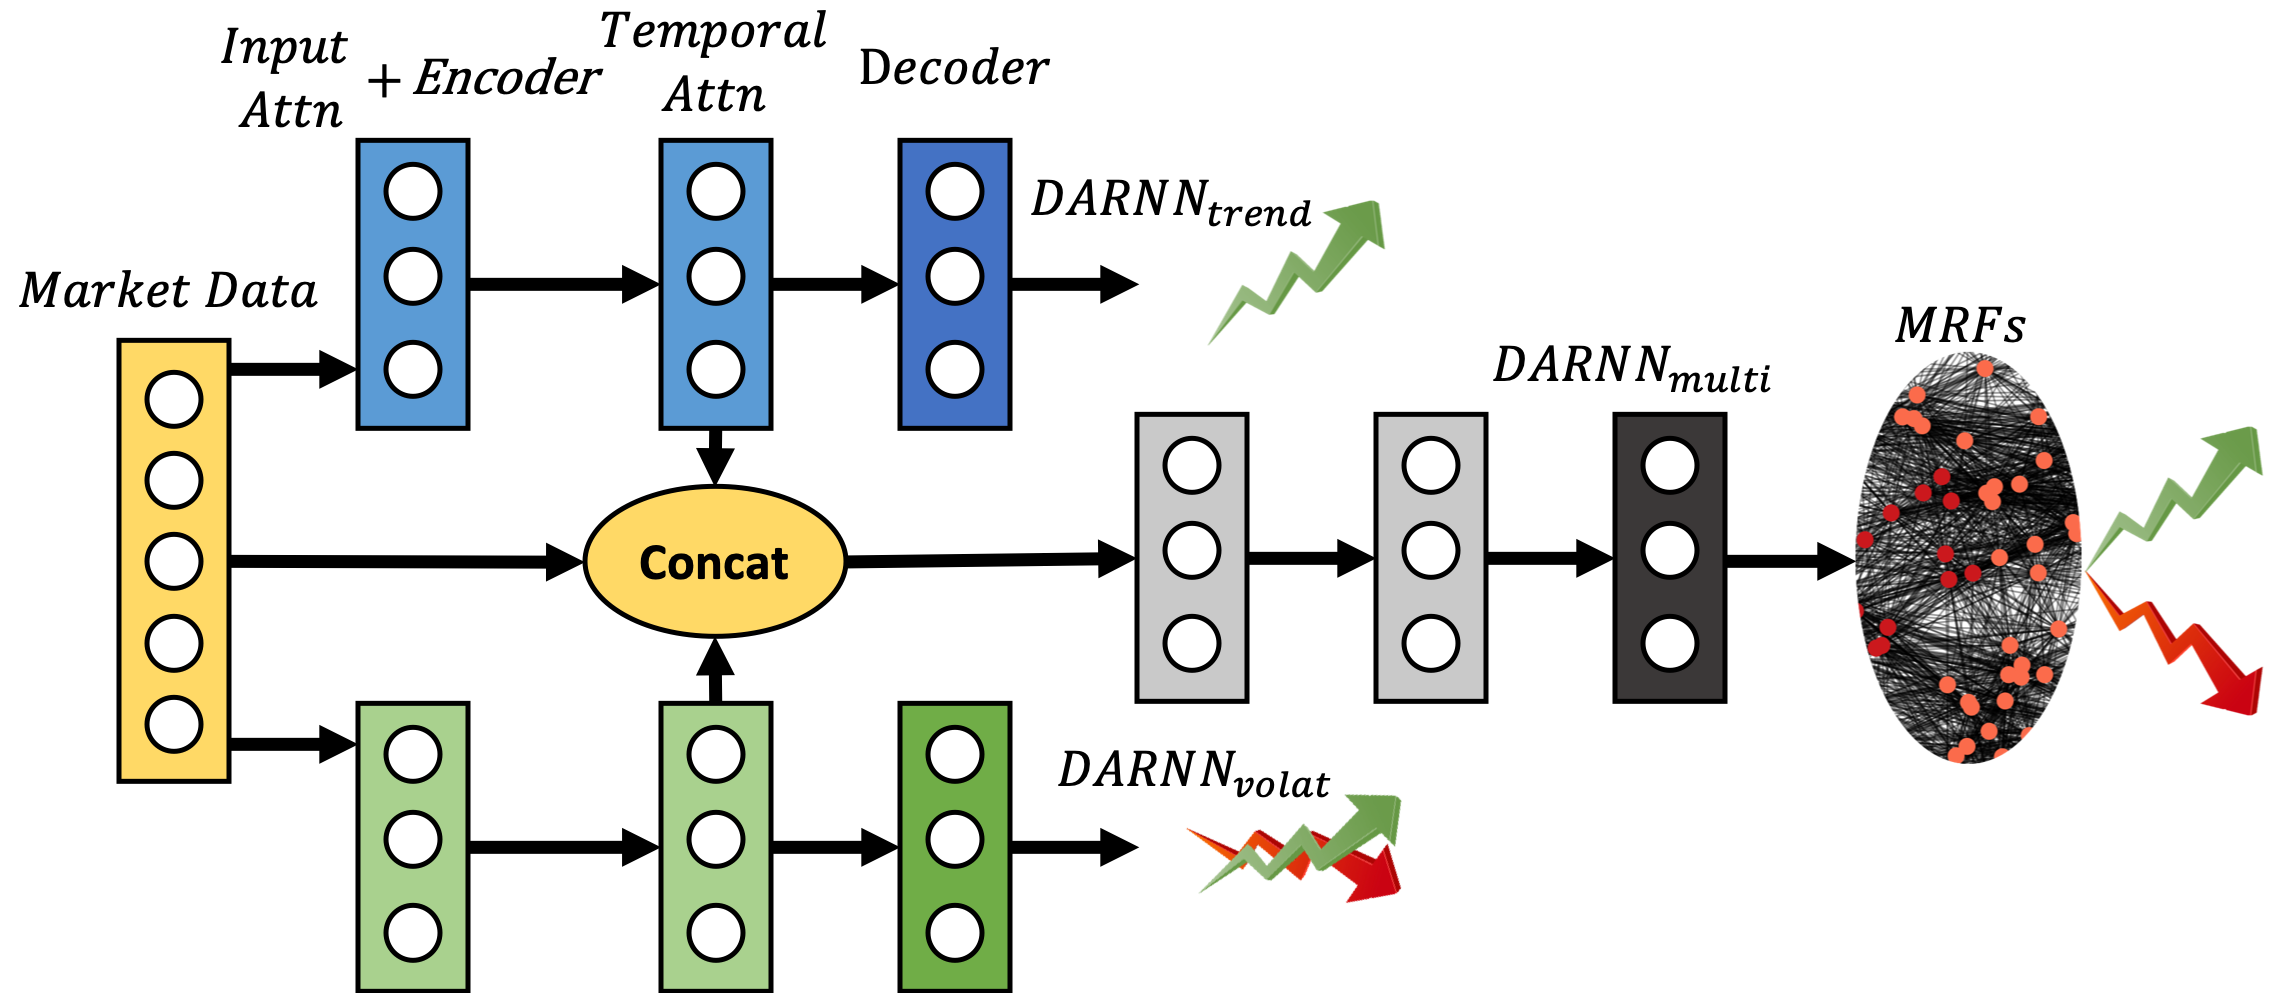
\includegraphics[width=1\columnwidth]{Part2/figures/mmplmrf.png}
  \caption{\label{fig:mrfrnn} Multi-task RNN-MRFs architecture. Note 
  that the output of $\text{DARNN}_{\text{multi}}$ only corresponds to one 
  node's unary feature in MRFs.}
\end{figure}

All three DARNN modules share the same raw market price data.
Here, we denote the time-series dataset as $\mX$ where
$\mX=(\vx_1,\vx_2,\dots,\vx_T)\in \sR^{N\times T}$. We use
$\vx^n=(x_1^n,x_2^n,\dots,x_T^n) \in \sR^T$ to denote a driving
series of $T$ time-steps and $\vx_t=(x_t^1,x_t^2 ,\dots
,x_t^N)\in \sR^N$ to denote a snapshot at time-step $t$ of all
$N$ features.

For both DARNN modules at the low level, the input is $\mX \in \sR^{5\times T}$
which contains $5$ exogenous driving series, \textit{i.e.}, opening price, low
price, high price, volume, amount and $1$ target series $\vy =
(y_1,y_2,\dots,y_T) \in \sR^T$. These two modules
aim to predict target series $y_{t+p}$ in the next $p$ time
steps:

$$\hat{y}_{t+p} = \text{DARNN}(y_1,\dots,y_{t},x_1,\dots,x_t)$$

The target series $\vy_{\text{trend}}$ of
$\text{DARNN}_{\text{trend}}$ is the closing price. The target series
$\vy_{\text{volat}}$ of $\text{DARNN}_{\text{volat}}$ is the
standard deviation of closing price over $M$ constant time-steps.
In our implementation we set $M=10$. We use Mean Squared Error
(MSE) as the loss function to train those two modules separately.

To construct the high level DARNN module, which aims to predict
the price movement, we concatenate context vectors $\vc_T$ from
each of low level DARNN module's encoder and raw market price
matrix as the input. The target series $\vy^{\text{binary}}$ is
constructed by the sign function $y_t^{\text{binary}} =
sign(y_{t+p}-y_t)$ where $y_t$ denotes closing price at time-step
$t$. We use cross-entropy as loss function to train the final
$\text{DARNN}_{\text{multi}}$. Logits (outputs before going
through \emph{softmax}) of $\text{DARNN}_{\text{multi}}$ are then
passed to Intra-clique Predictor as unary features.

In order to train MMPL together with MRFs in an end-to-end
manner, we follow the subgradient method proposed by
\citename{witoonchart2017application}. Since our inner loop
proposed in section~\ref{sec:mrflssvm_learning_algo} is actually
a latent structural SVM. Only gradients of parameters and feature
functions need to be updated. In our framework, outputs of
MMPL (Logits of $\text{DARNN}_{\text{multi}}$) are only used as unary features in MRFs' energy functions,
our back-propagation rules can be defined by taking derivative of the objective function \textit{w.r.t} $\vw^U$  defined in
~\eqref{eq:mrflssvm_object}:

\begin{align}
  \label{eq:der_w}
  \frac{\partial L}{\partial \vw^U} = \psi^U(y)-\psi^U(y^*)
\end{align}

\noindent where $y$ is the ground-truth label and $y^*$ is
inferenced label. $\psi^U$ is unary feature
function described in section~\ref{sec:llep}, here it denotes
logits calculated from $\text{DARNN}_{\text{multi}}$. $\vw^U$ is
unary parameter defined in energy function~\eqref{eq:energyfunction_UPH}.
Equations \eqref{eq:der_w} can be directly plugged
into sub-gradient algorithm proposed in \cite{witoonchart2017application}.
Other configurations stay the same with their algorithm.

\subsection{Intra-clique Predictor}
\label{sec:srp}

In this section, we show how to construct an ``Intra-clique
Predictor" with MRF-LSSVMs to model lead-lag relationships and
address the other two challenges as mentioned in the
introduction. Specifically, each stock is treated as a node in
MRFs and each stock's group with lead-lag relationships is
treated as a maximum clique in MRFs. We use a pre-defined
industry classification list \cite{ths} as the prior domain
knowledge of each maximum clique for each stock. By using a
weighted version of higher order functions, stocks have higher
weights in the above list can be seen as leading stocks, and vice
versa. However, in our implementation, we use logits from MMPL as
unary function and weighted lower linear envelopes as higher
order function to encode lead-lag relationships. Pairwise
features are excluded. Finally, the complexity of modeling
dynamics between leading and lagging stocks becomes encouraging
consistency over large cliques under weighted lower linear
envelope potentials. Log- its from hierarchical RNN networks are
used as unary features in MRFs. By minimizing the energy function
which contains both unary and higher order features, we can
predict each stock's future price movement by jointly considering
individual market price trends together with lead-lag
relationships.


The detail of the optimization algorithm is summarized in
\algref{alg:learning_app}. As we mentioned in
\appref{sec:train_detail}, although we proposed an end-to-end
subgradient algorithm is section \ref{sec:mmpl}, MRFs updated by
such algorithm take too many iterations to converge. Therefore,
we propose a two-stage training procedure. At first stage, MMPL
and MRFs are trained separately. Therefore, MRFs can take
advantage of the efficient latent structural SVM and converge in
a polynomial number of iterations. After all those models are
converged, we then combine them together to conduct end-to-end
training. Note that the CCCP Inner Loop in
\algref{alg:learning_app} is actually solving standard structural
SVM problem. Therefore, at the second stage, we use subgradient
algorithm proposed in section~\ref{sec:mmpl} to replace the CCCP
Inner Loop. Other settings remain the same.


\begin{algorithm}[h]
  \begin{algorithmic}[1]
    \STATE{Set $MaxIter = 100$}
    \STATE{ {\bf input} training set $\{\vy_i\}_{i=1}^{n}$, regularization constant $C > 0$,
      and tolerance $\epsilon \geq 0$}
    \STATE{Initialize $\vtheta$ using \algref{alg:init_theta}}
    \REPEAT \STATE{CCCP Outer Loop}
    \STATE{Set $iter = 0$}
    \FOR{each training example, $i = 1, \ldots, n$}
    \STATE{compute $ \vz_i^*=\argmax_{\mathbf{z} \in \mathcal{Z}}
      \theta \cdot \psi(\mathbf{y}_i,\mathbf{z}) $}
    \ENDFOR

    \STATE{ {\bf initialize} active constraints set ${\cal C}_i = \{ \}$ for all $i$}
    \REPEAT \STATE{CCCP Inner Loop}

    \STATE{solve the quadratic programming problem in
      equation~\ref{eq:mrflssvm_object} with respect to active
      constraints set ${\cal C}_i$ for all $i$ and concavity constraints
      $A\vtheta\geq \epsilon$ to get
      $\hat{\vtheta}$ and $\hat{\vx_i}$}

    \FOR{each training example, $i = 1, \ldots, n$}
    \STATE{compute $\hat{\vy_i},\hat{\vz_i} = \argmin_{\vy}
      E(\vy,\vz; \hat{\vtheta}) - \Delta(\vy, \vz, \vy_i)$}
    \IF{$\hat{\xi}_i + \epsilon \!<\! \Delta(\hat{\vy_i},
      \hat{\vz_i}, \vy_i) -
      E(\hat{\vy_i},\hat{\vz_i}; \hat{\vtheta}) + E(\vy_i, \vz_i^*; \hat{\vtheta})$}
    \STATE{${\cal C}_i \leftarrow {\cal C}_i \cup \{{\vy}_i^\star\}$}
    \ENDIF
    \ENDFOR
    \UNTIL{no more violated constraints}
    \STATE{ {\bf return} parameters $\hat{\vtheta}$}
    \STATE{Set $iter = iter+1$}

    \UNTIL{$iter\geq MaxIter$}
    \STATE{ {\bf return} parameters $\hat{\vtheta}$}
  \end{algorithmic}
  \caption{\label{alg:learning_app} Learning lower linear envelope
    MRFs with latent variables.}
\end{algorithm}

Empirically, the more evenly distributed of $W_c(Y_c)$ where
$c\in\cal C$ on $x$ axis, the more rich representation (number of
linear functions) the energy function should have. In order to
initialize $\vtheta$, we first determine the x-coordinate of
sampled points $sp$. Then we sample its y-coordinate from a
uniform distribution ${\cal
  U}(\text{upbound},\text{upbound}-0.5)$ to add some randomness
in our initialization as well as maintain concavity. Linear
parameters $a_k$ and $b_k$ are later calculated using those
sampled points $sp_k$ and $sp_{k-1}$. At last we encode
$\{a_k,b_k\}_{k=1}^K$ into $\vtheta$ using
equation~\eqref{eq:llsvm_param}. This algorithm is summarized in
\algref{alg:init_theta}.

\begin{algorithm}[h]
  \begin{algorithmic}[1]
    \STATE{$gap=\frac{1}{K}$, $a_1={\cal U}(0,1e6)$, $b_1=0$,
      $sp_1=(0,0)$, $w_0=0$, $counter=2$} \FOR{each
      clique $c\in \cal C$} \STATE{Compute weighted clique value
      $w_c=W_c(y_C)$} \IF{$w_c-w_{c-1}>gap$}
    \STATE{$upbound = a_{counter}w_c+b_{counter}$\\
      $sp_{counter}=(w_c,{\cal U}(upbound-0.5,upbound))$\\
      Calculate $a_{counter}$ and $b_{counter}$ using
      $sp_{counter-1}$ and $sp_{counter}$\\
      $counter=counter+1$}
    \ENDIF
    \ENDFOR
    \STATE{If $counter<K$, remaining $a$s and $b$s are all set to
      be $a_{counter}$ and $b_{counter}$} \STATE{Calculate
      $\vtheta$ using $\{a_k,b_k\}_{k=1}^K$}
  \end{algorithmic}
  \caption{\label{alg:init_theta} Empirical initialization
    algorithm for $\vtheta$}
\end{algorithm}



\section{Dataset and Model Settings}
\label{sec:dataset}

In this section, we first introduce 3 stock datasets. Then, we
introduce the parameter settings for our model and training
details. Finally, we select four evaluation metrics and use them
to demonstrate the effectiveness of our proposed model by
comparing to several baseline approaches.

To demonstrate the effectiveness of higher order consistency, we
choose three exclusive and the most famous stock indexes on Chinese
stock market to build our input datasets. Their index codes are:
CSI (China Securities Index) 200, CSI 300 and CSI 500 which
contain 200, 500 and 300 constituent stocks respectively. The CSI
300 index selects most liquid A-share stocks. It aims to reflect
the overall performance of China A-share market. The CSI 200 and
500 indexes aim to reflect the overall performance of mid-to-large
and small-to-mid capital A-shares respectively.

All these indexes are exclusive and are refined on a yearly
basis. In this paper, we use fixed versions on 30-JAN-2015. We
then collect their constituent stocks' minute-level data from
05-JAN-2015 to 29-DEC-2017. On Chinese stock market each trading
day has 4 trading hours. So there are 240 samples (minutes) for
each normally traded stock on each day. Each sample contains 6
features: opening price, high price, low price, closing price,
volume, and amount. \footnote{During this period, there are some
  stocks de-listed (SZ000024, SH600485, SH600832 in CSI 200;
  SZ000693, SZ000748, SZ000982 in CSI 500; SH600485, SH600832,
  SZ000024, SH601299 in CSI 300). Therefore, in total we collect
  197, 497 and 296 stocks during this period respectively.} For
each stock, the first $80\%$ days are used to construct the
training set and the last $20\%$ days are used as test set.
Approximately training set and test set contain $33.6$ million
and $4.2$ million samples, respectively. $49.5\%$ of them are
positive movements, $0.3\%$ of them stay unchanged and $50.2\%$
of them are negative movements. For binary classification task,
we follow \citename{mitchell2001characteristics}'s approach and
label all positive movement samples $1$ and $0$ for the other
samples. More labeling details are described in appendix
\ref{sec:train_detail}.

\begin{table}[H]
\centering
\small
\caption{Technical Indicators Selection}
\begin{tabular}{|c|c|} \hline
  Category&Indicator Name\\ \hline
  Momentum& Awesome Oscillator, Money Flow Index\\ \hline
  Volume& \makecell{Chaikin Money Flow\\ On-balance volume mean}\\ \hline
  Volatility& Bollinger Bands (Upper and Lower Bands)\\ \hline
  Trend& \makecell{Average Directional Movement Index\\Moving Average Convergence Divergence}\\ \hline
\end{tabular}
  \label{tab:ta}
\end{table}
To demonstrate the benefits of multi-task RNN over manually designed
technical indicators, we construct technical
indicators datasets. We select 8 most popular indicators, 2 from each
category~\cite{kirkpatrick2010technical} shown in Table
\ref{tab:ta}. In implementation, we use open source package
\emph{Technical Analysis Library in
  Python\footnote{https://github.com/bukosabino/ta}} to calculate
those indicators and all hyperparameters are using package's
default settings without any prior expert knowledge involved
with. After technical indicators calculation, these 8 new
features are concatenated to above market price dataset (5
features at each minute). So the final input dataset for each
single task model contains 13 features in total. Before feeding
into models, we normalize each stock with \emph{z-score} function
using standard deviation and mean calculated in the training set.

For brevity, we denote market price dataset which only contains
$5$ features as \textbf{Market} and the concatenated $13$
features dataset as \textbf{Indicator}. As discussed in
section~\ref{sec:mmpl}, closing price at time $t$ can be directly
used as regression target for $\text{DARNN}_{\text{trend}}$.
Standard deviation of closing price with a window size of $10$ is
used as regression target for $\text{DARNN}_{\text{volat}}$. The
dimensions of hidden state and cell state are fixed as 32 for
$\text{DARNN}_{\text{trend}}$ as well as
$\text{DARNN}_{\text{volat}}$, and 128 for
$\text{DARNN}_{\text{multi}}$. More training details are
described in appendix \ref{sec:train_detail}.

\section{Results}
\label{sec:res}

In order to demonstrate the effectiveness of our framework, we
compare 3 baseline methods, \textit{i.e.},
LSTM~\cite{hochreiter1997long}, attention based LSTM
Encoder\_Decoder~\cite{attention}, and DARNN~\cite{qin2017dual}
on 3 different Chinese Securities Indexes with and without
technical analysis indicators as inputs. Results are summarized
in Table~\ref{tab:result}. All results are reported over the test
sets. We select four metrics (Accuracy, Precision, Recall and F1
Score) as evaluation metrics to justify the effectiveness of the
proposed approach. They are calculated by collecting all
predicted labels of constituent stocks in each CSI index.

\begin{figure}[t]
  \centering
  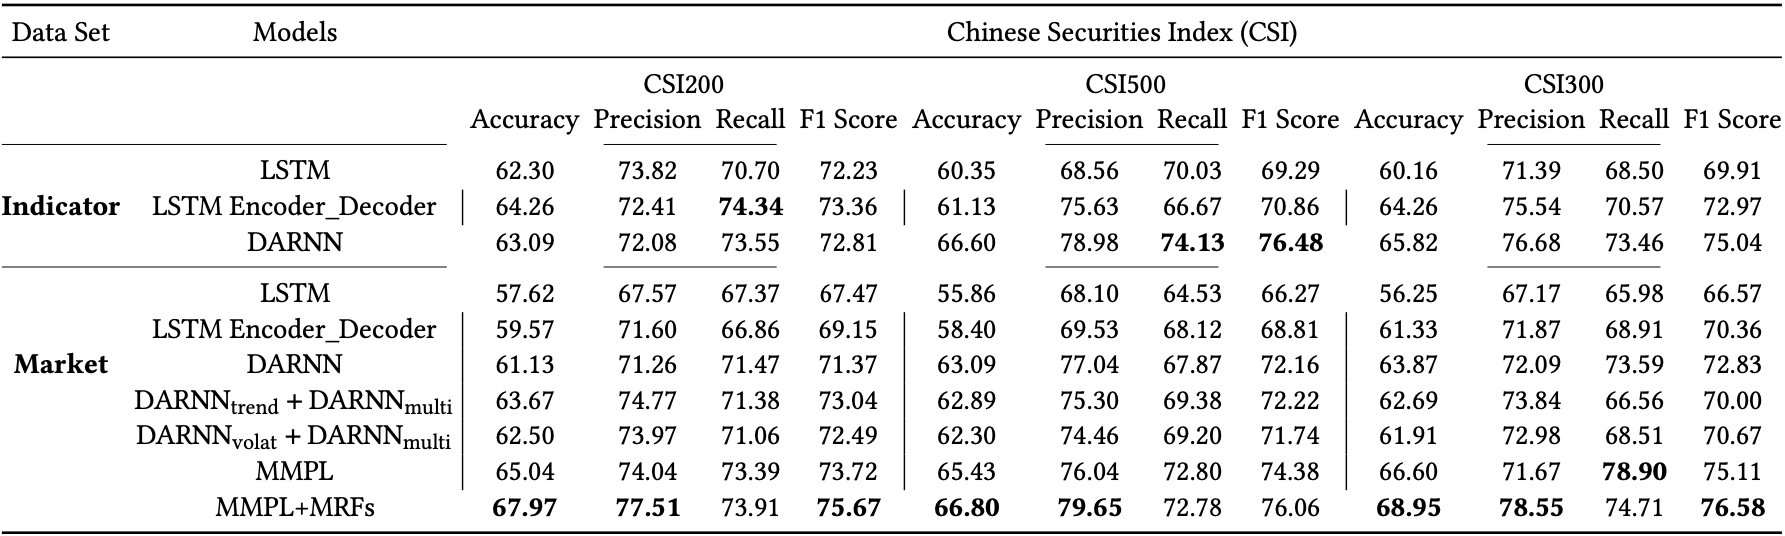
\includegraphics[width=1\columnwidth]{Part2/figures/table_results.png}
  \caption{\label{tab:result} Results: baselines and ablation
    studies. All models have a window size (lag steps) of 20 and
    predict price movement label at the next time step.}
\end{figure}


\subsection{Effectiveness of multi-task framework}

As mentioned earlier, to demonstrate effectiveness of multi-task
framework, we use \textbf{Indicator} dataset, which contains both
market price data and technical analysis indicators as inputs for
baseline approaches and \textbf{Market} dataset which only
contains market price data as inputs for MMPL (multi-task RNN) as
well as baseline methods. For DARNN, we use a hidden size of
$128$. MMPL's configuration is described in
section~\ref{sec:multi_train}. As we can see in
Table~\ref{tab:result}, single task models (LSTM, LSTM
Encoder\_Decoder, DARNN) tested on \textbf{Market} dataset
(without technical analysis indicators as inputs) generally have
worse performance with all 4 metrics. In particular, performance of
DARNN models tested on \textbf{Indicator} dataset is consistently
better than the ones on \textbf{Market} dataset. This proves that
even with hand-crafted features, deep learning models can still
benefit from diversified and complementary features.

To test the effectiveness of multi-task framework, we conduct
ablation study with only one low-level task (\quad
$\text{DARNN}_\text{trend}$ \quad or \\
$\text{DARNN}_\text{volat}$) together with the high-level task
module $\text{DARNN}_\text{multi}$. Results indicate that these
two variants have comparable or slightly worse result than DARNN
on \textbf{Market}. This may because single task model does not
provide diversified features while have more parameters than
DARNN. Finally, MMPL outperforms all single task models and
baseline methods on \textbf{Market}. This suggests that
diversified and complementary tasks can help MMPL extract
effective features. Specifically, by comparing MMPL and DARNN on
\textbf{Market} as well as \textbf{Indicator}, we can see that
MMPL generally outperforms DARNN on CSI200 and CSI300 indexes and
is slightly worse than DARNN on \textbf{Indicator} of CSI500
index. We can conclude that by using multi-task RNNs, we can
extract better or at least comparable features compared with
hand-crafted features.

\subsection{Effectiveness of higher-order MRFs}
In Table~\ref{tab:result}, we can observe that MMPL-MRFs
framework consistently outperforms other baselines on all 3 CSI
index constituent stocks. It shows evidence that higher-order
energy function can help with encoding clique level consistency
thus improving overall prediction performance. One interesting
point to note is that the recall rate of MMPL-MRFs is constantly
lower than other baselines. This can be seen as a trade off
between accuracy and recall rate. However, it is worth to mention
that for stock price movement prediction, high accuracy and
precision are much preferred than recall rate. Another
interesting phenomenon is that MMPL-MRFs gives more improvement
on CSI200 and CSI300 while less improvement over DARNN trained
with technical analysis indicators on CSI500. One possible reason
is that CSI200 and CSI300 select most liquid and representative
stocks in Chinese stock market. Those stocks exhibit much
stronger and higher order consistency than illiquid stocks.
CSI500 selects small-mid capital stocks which are less liquid and
contains much more noisy movements.

In the training stage, our algorithm converges in 4 to 19
CCCP outer loops. The average inference time of graph-cut
algorithm is 34 seconds.

\subsection{Visualization of higher-order consistency}

In order to further investigate higher-order MRFs' effectiveness,
we design a heat-map to visualize CSI300 index intra-clique
higher-order relationship in figure~\ref{fig:consistency}.

\begin{figure*}[t]
  \centering
  \setlength{\tabcolsep}{20pt}
  \begin{tabular}{cc}
  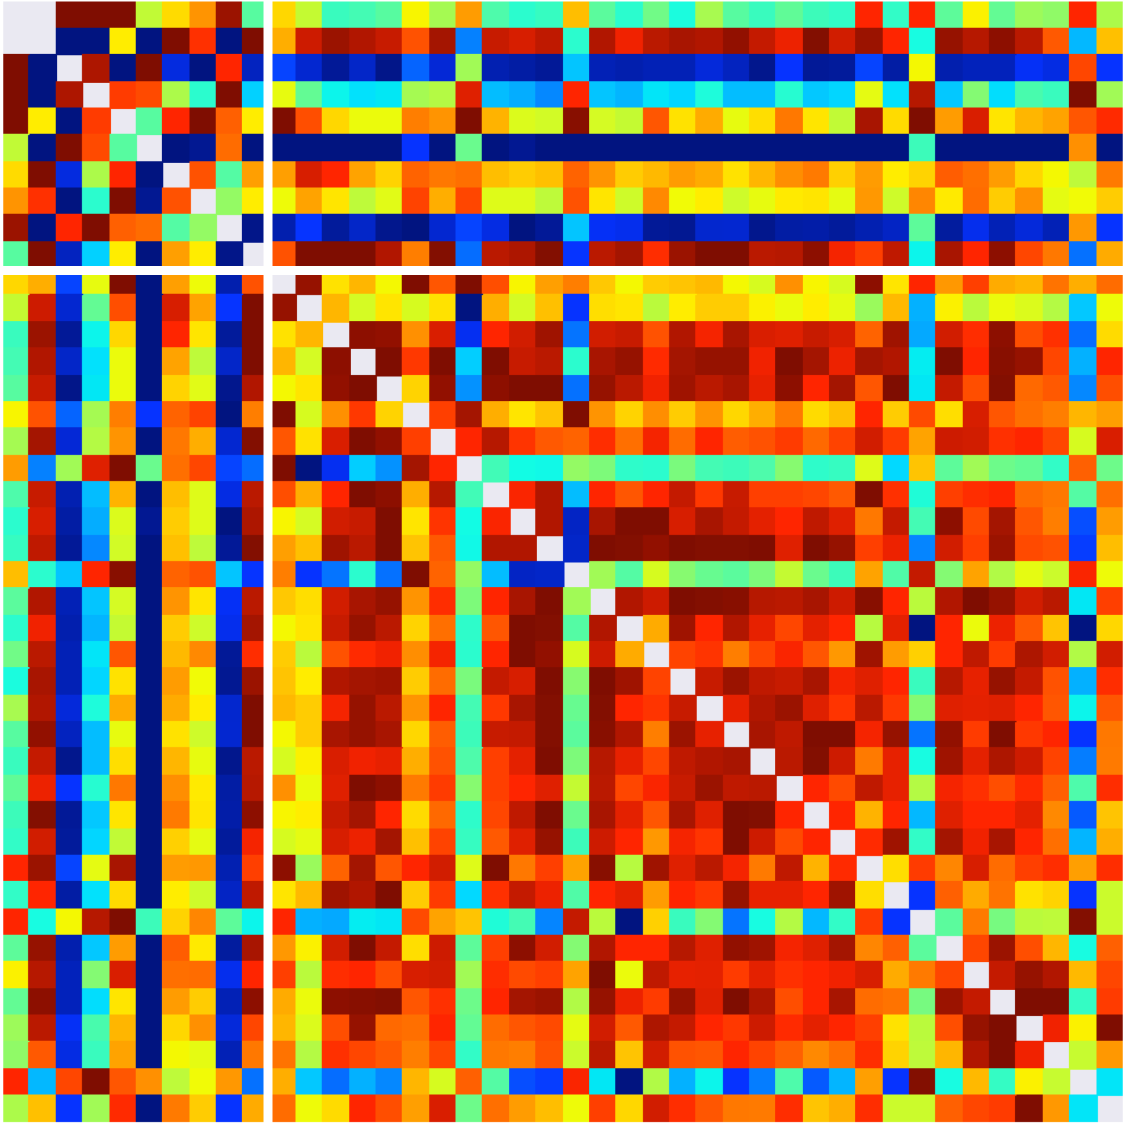
\includegraphics[width=0.4\columnwidth]{Part2/figures/gt.png}&
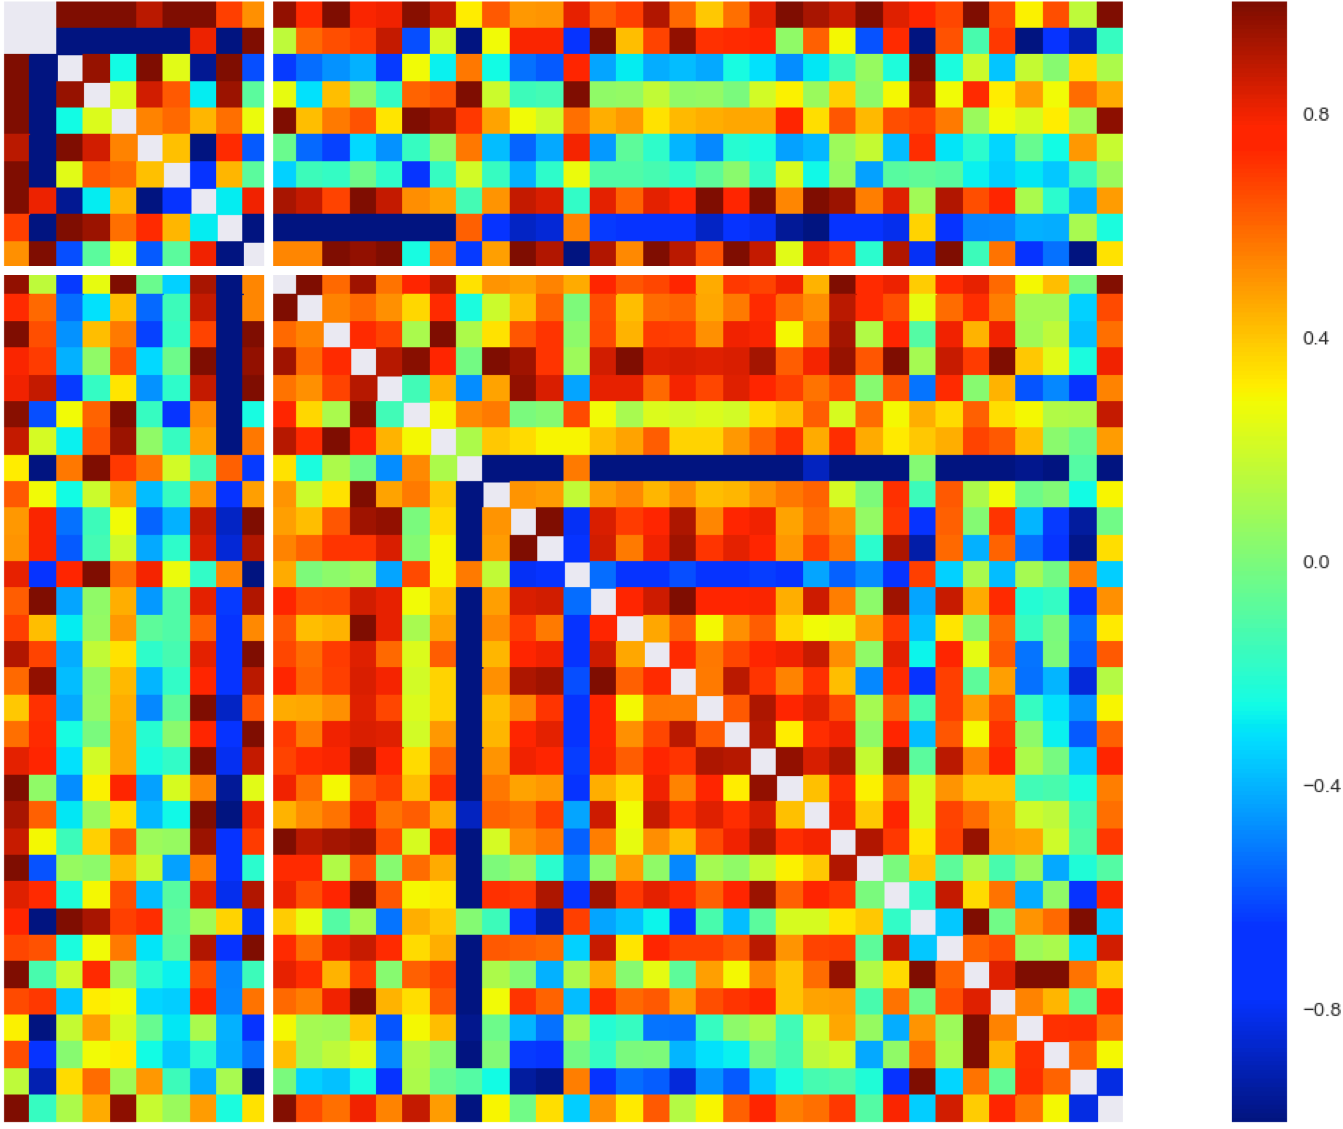
\includegraphics[width=0.48\columnwidth]{Part2/figures/mmpl.png}\\
{\small (a) Ground-truth} & {\small (b) MMPL }\\
    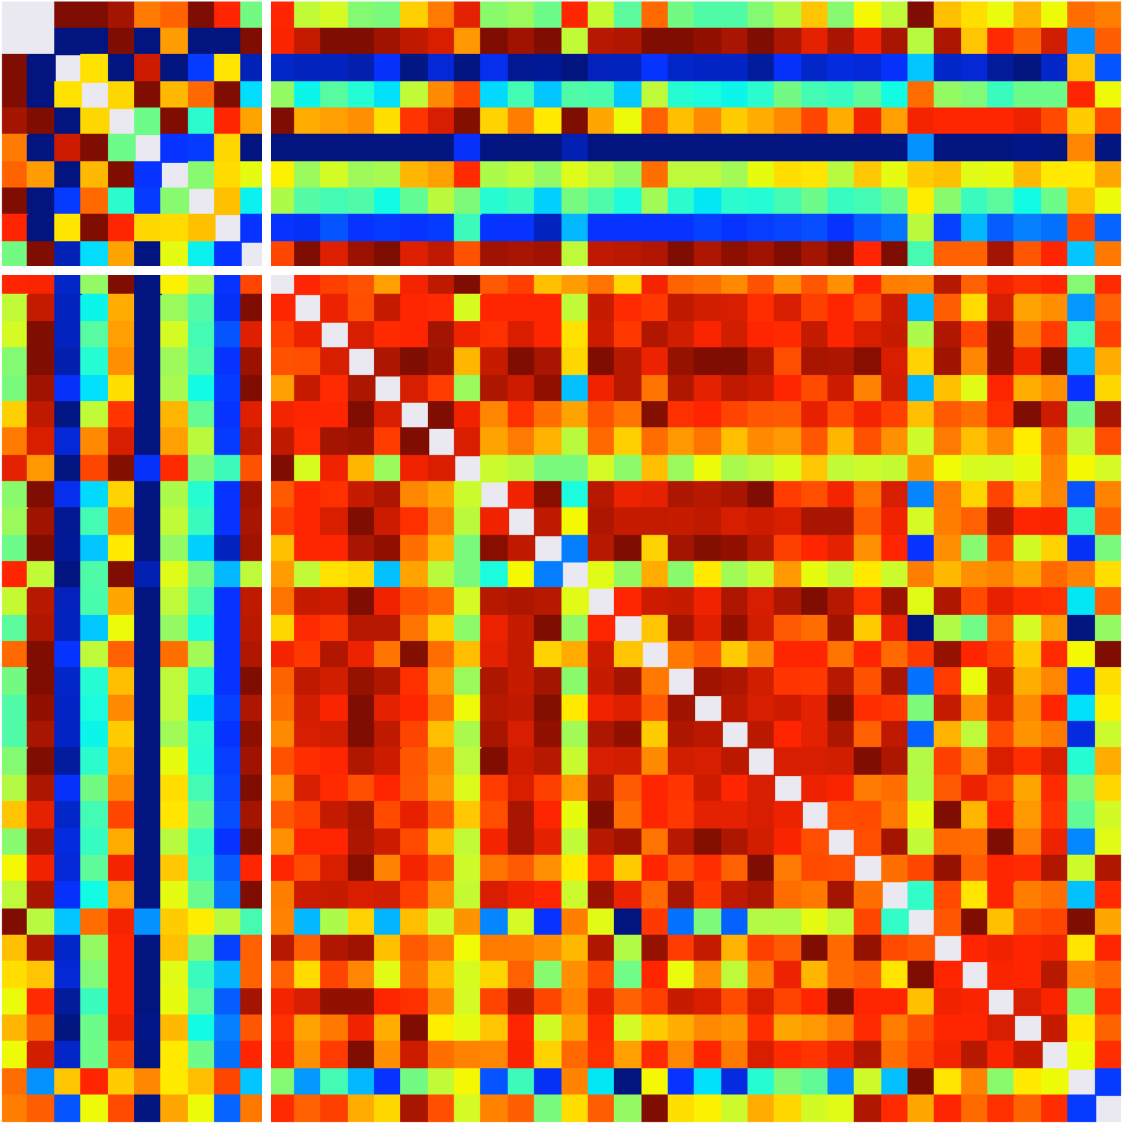
\includegraphics[width=0.4\columnwidth]{Part2/figures/mrf.png}\\
{\small (c) MMPL-MRFs}\\
  \end{tabular}
  \caption{\label{fig:consistency} Higher order consistency
    visualization. (a) is calculated
    directly from ground truth labels on test set.
    (b)
    is calculated using predicted labels of MMPL without MRFs on the
    test set.
    (c), we use predicted labels of
    MMPL-MRFs on test set as inputs.}
\end{figure*}

We first select two sectors: nonferrous metal sector, which
contains 10 constituent stocks, and infrastructure sector, which
contains 35 constituent stocks from CSI300 index \footnote{These
  two sectors are selected only because painting many sectors in
  one figure would be too messy to interpret and those two
  sectors have appropriate clique size (number of stocks) for
  visualization. Conclusions from these two sectors also apply to
  other sectors}. We then measure consistency level between each
two of these constituent stocks. In order to capture their
temporal relationship, we propose a novel consistency measure
which is calculated on temporal intervals.
% Let $\C\in\{\text{Nonferrous Metal},\text{Infrastructure}\}$
% denotes one clique. $\by_c=\{\by_i \in \C\}$ denotes a set of
% time-series $\by_i^T=\{y_i^1,y_i^2,...,y_i^T\}$ for all stocks

Let $\vy_i^T=\{y_i^1,y_i^2,...,y_i^T\}$ denotes time-series for
stock $i$. $y_i^t\in \{0,1\}$ is the binary price movement label
at time $t$. We segment time-series $\vy_i^T$ into
$N=\lceil\frac{T}{P}\rceil$ non-overlapping intervals
$\{y_i^n,y_i^{n+1},...,y_i^{n+P}\}$ with fixed length $P$. For
any two stocks $i$ and $j$, we calculate the difference
$d_{ij}^n=\sum_n^{n+P}{y_i^n}-\sum_n^{n+P}{y_j^n}$ of how many
times positive price movement happen in the $n$-th time interval
in each stock. Then the consistency level $c_{ij}$ between stocks
$i$ and $j$ can be calculated via a $\ell_1\text{norm}$:
$$c_{ij}=-\|\mathbf{d}_{ij}\|_1$$
\noindent where
$\mathbf{d}_{ij}=\{d_{ij}^1,d_{ij}^2,...,d_{ij}^N\}$. We
normalize $c_{ij}$ into interval $[-1,1]$. Each entry in
figure~\ref{fig:consistency} denotes a consistency level measure
$c_{ij}$. The larger the $c_{ij}$ is, the higher of consistency
level between stock $i$ and stock $j$, the color of corresponding
entry is closer to red, and vice versa. As we mentioned, the average duration of information
arrival-conduction-integration-release process is 4.04 minutes~\cite{fangyan2012}.
Since which stock is leading at each time interval is elusive, we
set $P=9$ when calculating consistency measures.

As we can see in Figure 4(a), there is a significant red square
area, which means ground-truth heat-map shows strong intra-clique
consistency. This is an evidence that higher-order relationships
do exist within clique of stocks. However, in Figure 4(b), the red
square area is fragmented into many little pieces. The whole
area's color is closer to blue when compared to ground-truth
heat-map, which means that MMPL captures little higher-order consistency.
The reason we still can observe a shape of red square
is that the accuracy of MMPL model on CSI300 is $66.6\%$.
However, we can still conclude that the accuracy of single MMPL
model mainly comes from unary features and it fails to capture
higher order consistency of different stocks belonging to the same clique.
On the contrary, even though MMPL-MRFs model's accuracy on CSI300
index is only $2.35\%$ better than MMPL model, we can observe
that heat-map Figure 4(c) is more close to ground-truth heat-map than
heat-map Figure 4(b). There is a much clear red square and the number of
small fragments in red area is also less than Figure 4(b). We can
conclude that MMPL-MRFs models learn to utilize both unary
features from MMPL as well as higher-order relationships encoded
in MRFs.

\section{Conclusions}
\label{sec:conc}

Here we show how to model individual stock price predictions
without hand-crafted features and encode lead-lag relationships
between stocks using weighted higher-order MRFs. A multi-task
neural network framework: Multi-task Market Price Learner (MMPL),
is proposed to automatically extract diversified and
complementary features from individual stock price sequences.
Features learned by MMPL are passed to a binary MRF with a
weighted lower linear envelope energy function to utilize
intra-clique higher-order consistency between stocks. An
efficient latent structural SVM algorithm is designed to learn
MRFs in polynomial time. Finally, the MRFs and MMPL are trained
end-to-end using the sub-gradient algorithm. Extensive
experiments are conducted on three major Chinese stock market
indexes, and the proposed MMPL-MRFs achieve the best accuracy on
all three indexes.

Our work provides a number of directions for future research. In
this work we proposed a multi-task recurrent neural network for
stock price prediction. While we directly use DARNN as a proof of
concept, other, more dedicated architectures are worthy of
exploration. As well as time series tasks, we can also
investigate how the latent SSVM framework performs on computer
vision tasks. Another interesting direction is to investigate the
implicit relationship between the expert-defined index list and
graph RNN~\cite{you2018graphrnn}, which could further help to
reduce the domain knowledge required by our framework.

\section{Training Details}
\label{sec:train_detail}

\subsection{Multi-task training}
\label{sec:multi_train}

To improve accuracy and reduce over-fitting, we add a drop out
layer between input layer and LSTM layer with a ratio of $0.2$.
We also clip and normalize gradients during back-propagation
stage with a maximum norm of $5.0$ to prevent gradient exploding
issue. As pointed out by \citename{lample2016neural}, the
question of ``when should the training schedule switch from one
task to another task?'' or ``should each task be weighted
equally?'' remains open. In our implementation, we follow the
proportional sampling approach described by
\citename{sogaard2016deep}. After a backward pass completed, we
randomly sample a new task as well as its batch data as the next
task to be trained. In practice, we use a proportion of
$[0.25,0.25,0.5]$ for three tasks respectively. This mechanism
helps multi-task model to avoid \emph{Catastrophic Forgetting}
phenomenon which means lower level model forgets learned
knowledge during higher level model back-propagation pass.

Even though we propose an end-to-end training algorithm for MMPL
and MRFs in section~\ref{sec:mmpl}, MRFs inference stage is still
too slow to be trained jointly with MMPL. To overcome this
difficulty, we implement a two stages training procedure. We
first add a \emph{softmax} layer on top of
$\text{DARNN}_{\text{class}}$ and train MMPL separately from
MRFs. We use \emph{Negative Log-likelihood} as the loss function.
At the second stage, after MMPL converge, we remove the
\emph{softmax} layer and re-train it together with MRFs. One
issue we must mention is that, even though we use binary MRFs
which can only predict positive / negative price movement, we
find there is a significant amount of time when stock price
remains no change. We find it benefits the performance a lot if
we treat the classification as a three classes problem rather
than a binary classification problem during the first stage.
Therefore, at the first stage, the \emph{softmax} layer will
output probability for three labels: \emph{negative movement},
\emph{no changes} and \emph{positive movement}. Since binary MRFs
still needs a two dimension input as part of unary energy
function, after the \emph{softmax} layer is removed, we add an
additional linear mapping layer between logits of MMPL and MRFs
at the second stage.

\subsection{End-to-end multi-task RNN-MRFs training}
\label{sec:mrf_train}

With converged MMPL and MRFs at hand, now we can go forward to
train them in an end-to-end manner. We only include pairwise
energy function through section~\ref{sec:srp} and
section~\ref{sec:opt} to show a general application of our
proposed algorithm. In the case of Chinese stock market, to our
best knowledge there is no public available definition of
pairwise relationship between stocks. Therefore, in our
implementation we only use unary and higher order energy
function. Each stock is then treated as a node in MRFs and each
stocks group which has lead-lag relationships is treated as a
maximum clique in MRFs. One benefit of MRFs clique is that we can
embed domain expert knowledge about industry classification as
maximum cliques into our model. We choose to use Tonghuashun
industry classification \cite{ths} in our model. One subtle but
crucial detail about modeling lead-lag effect lies in
equation~(\ref{eqn:potential2}). Recall that $W_{\!c}(\vy_c) =
\sum_{i \in c} w_i y_i$ with $w^c_i \geq 0$ and $\sum_{i \in c}
w^c_i = 1$ which are weights for stocks in each clique.
Therefore, leading stocks should have a higher weights while
lagging stocks should have lower weights. In our implementation,
we use constituents' weight defined in CSI200, CSI500 and CSI300
as their weights in equation~(\ref{eqn:potential2}) and normalize
them to ensure the summation equals $1$.



%%% Local Variables:
%%% mode: latex
%%% TeX-master: "../thesis"
%%% End:
